%
% Chapter 3
%

\chapter{OBJECTIVES AND FUTURE WORK}
This chapter outlines the research objectives and proposed future work. 

\section{Research Objectives}
The overall focus of this study is the development of plasma fairing technology, however, much has yet to be accomplished before this technology is flight ready. To this end, the complex ND G550 geometry will be divided into two sub-systems: 1) main-strut-door assembly and 2) the shock-strut-torque-arm assembly. Flow control strategies will be explored for each of these subsystems varying plasma actuator configurations. Finally, the acoustic effects of the applied flow control will be characterized.

%\begin{figure}
%	\begin{center}
%		\centerline{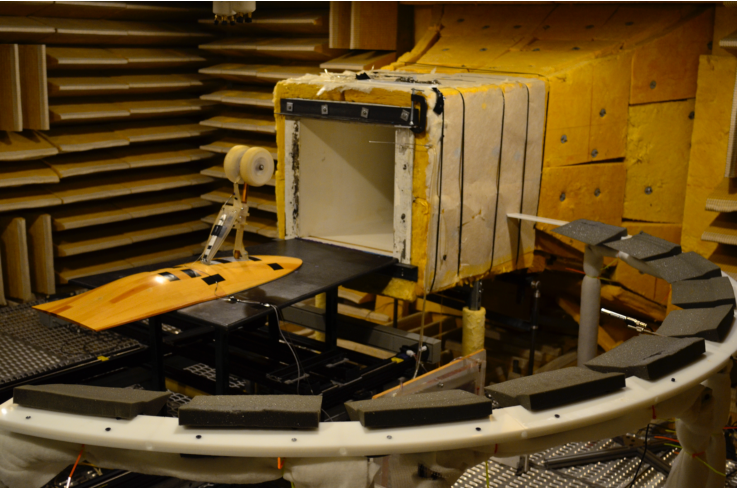
\includegraphics[scale=1.0]{figures/arraypic}}
%		\caption{Photograph of the polar array installed in the ND AWT.}
%		\label{fig:arraypic}
%	\end{center}
%\end{figure}

While the ultimate purpose of this research is the reduction of noise on aircraft landing gears, the objectives of this study will emphasize the documentation of the most successful flow control strategies and underlying physical mechanisms responsible. Regardless if noise reduction is actually achieved, there is much to be gained through a deeper understanding of the effects of various flow control strategies on noise generation.

\section{Proposed Future Work}
The following sections detail the experiments that will be performed to accomplish the outlined research objectives.

\subsection{Plasma Actuator Configuration}
Recall from Figure \ref{fig:mod1b}, the plasma fairing that has been retrofitted to the ND G550 nose landing gear model. Plasma actuators will be fixed to this partial fairing geometry. Both spanwise and PSVG configurations will be explored. The effects of geometric parameters will be examined such as spanwise actuator azimuthal placement and upstream versus downstream forcing. Also, the effects of plasma actuation parameters such as voltage, frequency, and interelectrode spacing (PSVGs only).

As parameters are varied the changes to the flow field will be documented using high speed flow visualization similar to that in Figure \ref{fig:flowvis}. Particle Image Velocimetry (PIV) will be performed to quantify these flow fields and calculate the effects on vorticity, as changes to vorticity can result in significant changes to the acoustic signature.

From the preliminary results cited in the previous chapter, a minor reduction in noise was observed when the main strut wake impingement was reduced on the downstream door. Unsteady pressure sensors will be used at various locations near the door's edge to quantify the effect of varying the parameter space of the plasma actuator. Both power spectral density and RMS pressure coefficient will be calculated.

\subsection{Noise Reduction Assessment}
The plasma actuator configurations deemed most likely to reduce noise will be selected based on the previous measurements. These configurations will then be tested on the model in the AWT facility. 
The polar array depicted in Figure \ref{fig:arraypic} will be used to measure magnitude and directivity of noise generated by baseline model and with plasma actuators installed. The difference in overall sound pressure level (OASPL) will also be calculated.
It is possible that iteration will be necessary to identify the most promising plasma actuator configurations, as reduction in unsteady pressure is not necessarily indicative of noise reduction of a similar magnitude. 
Finally, phased-array noise source identification will be performed to reveal where on the ND G550 model, flow control was most effective. Analysis of the underlying mechanisms will also be presented, by correlating aerodynamic and acoustic data.

\section{Conclusion}
While preliminary experiments demonstrate only a marginal effect of plasma flow control on noise reduction, flow visualization suggests a ``path forward'', by focusing on the elimination of wake impingement of the main strut on the door. Additionally, studies performed on the shock strut and torque arm geometries confirm that this flow control strategy may apply to other locations of aircraft landing gear. Several plasma actuator configurations will be utilized while documenting both the aerodynamic and acoustic effects. This study will focus on the underlying physical mechanisms responsible for noise production on the ND G550 nose landing gear model and the effects of flow control via plasma actuation.